% REPORT FOR PROJECT1 SF2565

\documentclass[a4paper,10pt]{article}

%%Packages	%%%	%%%	%%%	%%%	%%%	%%%	%%%
\usepackage{amsmath,framed}
\usepackage[latin1]{inputenc} 	
\usepackage{listings}
\usepackage{xcolor}
\usepackage{graphicx}
\usepackage{placeins}

%%Settings	%%%	%%%	%%%	%%%	%%%	%%%	%%%
\renewcommand{\d}{\text{d}}
\newcommand{\e}{\text{e}}
\newcommand{\ve}{\mathbf}
\newcommand\numb{\addtocounter{equation}{1}\tag{\theequation}}

\setlength\fboxsep{1.2mm}
\setlength\fboxrule{0.5mm}

\lstset { %
  language=C++,
  backgroundcolor=\color{black!3},	% set backgroundcolor
  basicstyle=\footnotesize,		% basic font setting
}

%%Margins	%%%	%%%	%%%	%%%	%%%	%%%	%%%
\usepackage{geometry}
\geometry{
  a4paper,
  left=40mm,
  right=40mm,
  top=40mm,
  bottom=40mm,
}

%%Header & Footer	%%%	%%%	%%%	%%%	%%%	%%%
\usepackage{fancyhdr}
\pagestyle{fancy}
\renewcommand{\headrulewidth}{1pt}
\rhead{Hanna Hultin, Mikael Perssson}
\lhead{P1 SF565}

\title{Project 1, SF2565}
\author{Hanna Hultin, TTMAM2 \\ Mikael Persson, TTMAM2}
\begin{document}
\maketitle

\subsubsection*{Task 1}
In this task we implemented the Taylor approximations for $\sin x$ and $\cos x$.
This was done by avoiding computing the factorials in the denumerators and the powers of $x$ in the numerators explicitly.
Consider the $2N$ degree Taylor polynomial for  $\cos x$
\begin{align*}
  \cos x &\approx p_c(x) = \sum_{n=0}^{N} (-1)^n \frac{x^{2n}}{(2n)!} \\ 
  \quad &= 1 + (-1) \frac{x^2}{2!} + (-1)^2 \frac{x^4}{4!} + \dots + (-1)^N \frac{x^{2N}}{(2N)!}
  \\
  &= 1 - \frac{x\cdot x}{2\cdot 1} \Big(1 - \frac{x \cdot x}{ 4 \cdot 3} \Big( 
  1 - \dots \Big(1- \frac{x \cdot x}{(2N)(2N-1)}\Big)\dots \Big).
\end{align*}
Hence, the polynomial may be evaluated backwords using the following scheme
\begin{align*}
  b_N &= 1-\frac{x \cdot x}{2N(2N-1)} \\
  b_n &= 1-\frac{x\cdot x}{2n(2n-1)}b_{n+1},\quad n = N-1,N-2,\dots,2,1 \\
  b_1 &= p_c(x).
\end{align*}
This is Horners' algorithm adjusted for the fact that each second term in the polynomial vanishes.
Similarly for $\sin x$ the polynomial may be computed up to degree $2N+1$ by
\begin{align*}
  b_N &= 1-\frac{x \cdot x}{2N(2N+1)} \\
  b_n &= 1-\frac{x\cdot x}{2n(2n+1)}b_{n+1},\quad n = N-1,N-2,\dots,2,1 \\
  x\cdot b_1 &= p_s(x).
\end{align*}
The algorithms above are implemented and the errors 
$|\cos x - p_c(x)|$ and $|\sin x - p_(x)|$ are 
investigated for a set of values of $x$.


\begin{table}[!ht]
\centering 
  \begin{minipage}[t]{105mm}
    \caption{
      Performance of the Taylor series implementation shown for selected values of 
      $x$ and $N$. The values of \texttt{sx} and \texttt{sTx} are the computed values
      from the \texttt{cmath} builtin function and the implemented Taylor polynomial to degree $2N+1
      for $\sin x$
      respectively,
      same for \texttt{cx} and \texttt{cTx} for $\cos x$.
    } 
    \label{TABtask1}
  \end{minipage}

  \vspace{5mm}
  \begin{tabular}{l l l l l l} 
    \texttt{x}&\texttt{N}&\texttt{sx} & \texttt{sTx} & \texttt{cx} & \texttt{cTx} \\
    \hline
    \texttt{-1}	& \texttt{1}	
    & \texttt{-0.84147098} & \texttt{-0.83333333} & \texttt{0.54030231} & \texttt{0.50000000}	\\
    \texttt{-1}	& \texttt{2}	
    & \texttt{-0.84147098} & \texttt{-0.84166667} & \texttt{0.54030231} & \texttt{0.54166667}	\\
    \hline
    \texttt{2}	& \texttt{1}	
    & \texttt{0.90929743} & \texttt{0.66666667} & \texttt{-0.41614684} & \texttt{-1.00000000}	\\
    \texttt{2}	& \texttt{2}	
    & \texttt{0.90929743} & \texttt{0.93333333} & \texttt{-0.41614684} & \texttt{-0.33333333}	\\
    \texttt{2}	& \texttt{5}	
    & \texttt{0.90929743} & \texttt{0.90929614} & \texttt{-0.41614684} & \texttt{-0.41615520}	\\
    \hline
    \texttt{10}	& \texttt{5}	
    & \texttt{-0.54402111} & \texttt{-1056.93923361} &\texttt{-0.83907153}&\texttt{-1296.79541446}\\
    \texttt{10}	& \texttt{10}	
    & \texttt{-0.54402111} & \texttt{2.76109093} & \texttt{-0.83907153} & \texttt{6.66456434}	\\
     \texttt{10}	& \texttt{15}	
    & \texttt{-0.54402111} & \texttt{-0.54412728} & \texttt{-0.83907153} & \texttt{-0.83942021}	\\
     \texttt{10}	& \texttt{20}	
    & \texttt{-0.54402111} & \texttt{-0.54402111} & \texttt{-0.83907153} & \texttt{-0.83907153}	\\
 
 

  \end{tabular}
\end{table}



\begin{table}[!ht]
\centering 
  \begin{minipage}[t]{105mm}
    \caption{
      Result for some selected values of $x$ and $N$.
    } 
    \label{TABtask1}
  \end{minipage}

  \vspace{5mm}
  \begin{tabular}{l l l l} 
    \texttt{x}&\texttt{N}&\texttt{sin err/N+1term} & \texttt{cos err/N+1term} \\
    \hline
    \texttt{-1}	& \texttt{1}	& \texttt{0.97651818} & \texttt{0.96725534} 	\\
    \texttt{-1}	& \texttt{2}	& \texttt{0.98623657} & \texttt{0.98233977} 	\\
    \texttt{-1}	& \texttt{5}	& \texttt{0.99525535} & \texttt{0.99452832} 	\\
    \texttt{-1}	& \texttt{10}	& \texttt{nan} & \texttt{nan} 	\\
    \hline 
    \texttt{1}	& \texttt{2}	& \texttt{0.98623657} & \texttt{0.98233977} 	\\
    \texttt{1}	& \texttt{5}	& \texttt{0.99525535} & \texttt{0.99452832} 	\\
    \hline
    \texttt{2}	& \texttt{2} 	& \texttt{0.94641382} & \texttt{0.93165191}	\\
    \texttt{2}	& \texttt{5}	& \texttt{0.98122925} & \texttt{0.97838354}	\\
    \hline
    \texttt{3}	& \texttt{3}	& \texttt{0.92270632} & \texttt{0.90649330}	\\
    \texttt{3}	& \texttt{5}	& \texttt{0.95852439} & \texttt{0.95235057}	\\
    \texttt{3}	& \texttt{10}	& \texttt{0.98513048} & \texttt{0.98392664}	\\
    \hline
    \texttt{5}	& \texttt{3}	& \texttt{0.80518429} & \texttt{0.76830018}	\\
    \texttt{5}	& \texttt{5}	& \texttt{0.89113977} & \texttt{0.87584989}	\\
    \texttt{5}	& \texttt{10}	& \texttt{0.95977271} & \texttt{0.95639607}	\\
    \hline
    \texttt{10}	& \texttt{3}	& \texttt{0.47425379} & \texttt{0.41141849}	\\
    \texttt{10}	& \texttt{5}	& \texttt{0.65781950} & \texttt{0.62076516}	\\
    \texttt{10}	& \texttt{10}	& \texttt{0.85443812} & \texttt{0.84340922}	\\
    \texttt{10}	& \texttt{15}	& \texttt{0.92187411} & \texttt{0.91747435}	\\
    \texttt{10}	& \texttt{20}	& \texttt{0.94971903} & \texttt{0.94954946}	\\
  \end{tabular}
\end{table}

\FloatBarrier
\subsubsection*{Task 2}
In this task we implement Adaptive Simpson Integration to integrate the function $f(x) = 1 + \sin \e ^{3x}$ between $a=-1$ and $b=1$. We use the functions \texttt{iSimpson} and \texttt{i2Simpson} to compute the approximate integrals named $I$ and $I_2$ in the project description. We implemented the Adaptive Simpson Integration in the function \texttt{asi}.

In \texttt{asi} we look at it as if we have a tree instead of recursion. We do not implement an actual tree structure, instead we just keep track of which node we are currently in. When we go to the left child of a node we change $b$ to $(a+b)/2$ and when we go to the right child we change $a$ to $(a+b)/2$ and we also half the tolerance for every child. We can also go up from a child to its parent by doing the reverse computations.

We start in the root node with number $1$ and then we go to the left child by using $leftnode = 2*node$ until we get that $\text{errest}<15*tol$, and then we found our first leaf. When we find a leaf we keep going up in the tree by using $parentnode = floor(0.5 * node)$ until we find the first even node, there we go up one more step and then to the right with $rightnode = 2*node+1$. From there we start going to the left again until we find another leaf. If we can not find an even node before the root node when we go up from a leaf, we have been through the whole tree and can stop. We get the approximate value of the integral by summing $I_2$ for each leaf of the tree.

In Figure \ref{fig: tree} we can see how we go through the tree in the case when $tol=0.01$. We start from the root and go down to the left until we reach the first leaf which is node 4. Then we go up to 2 and down to 5 again which also is a leaf. Then we go up to 2, up to 1, down to 3, down to 6 and we found another leaf. Then up to 3 again, down to 7, down to 14 and we found another leaf. Then we go up to 7 again, down to 15, down to 30, down to 60 and we found another leaf. So we go up to 30 and down to the next leaf 61. Then up to 30, up to 15, down to 31 and down to the next leaf 62. Back to 31 and down to our last leaf 63. Then we go up to 31, up to 15, up to 7, up to 3, up to 1 and since we have not found a single even node (63,31,15,7,3,1 all uneven) we have gone through our whole tree and are done.

\begin{figure}[h!]
	\centering
	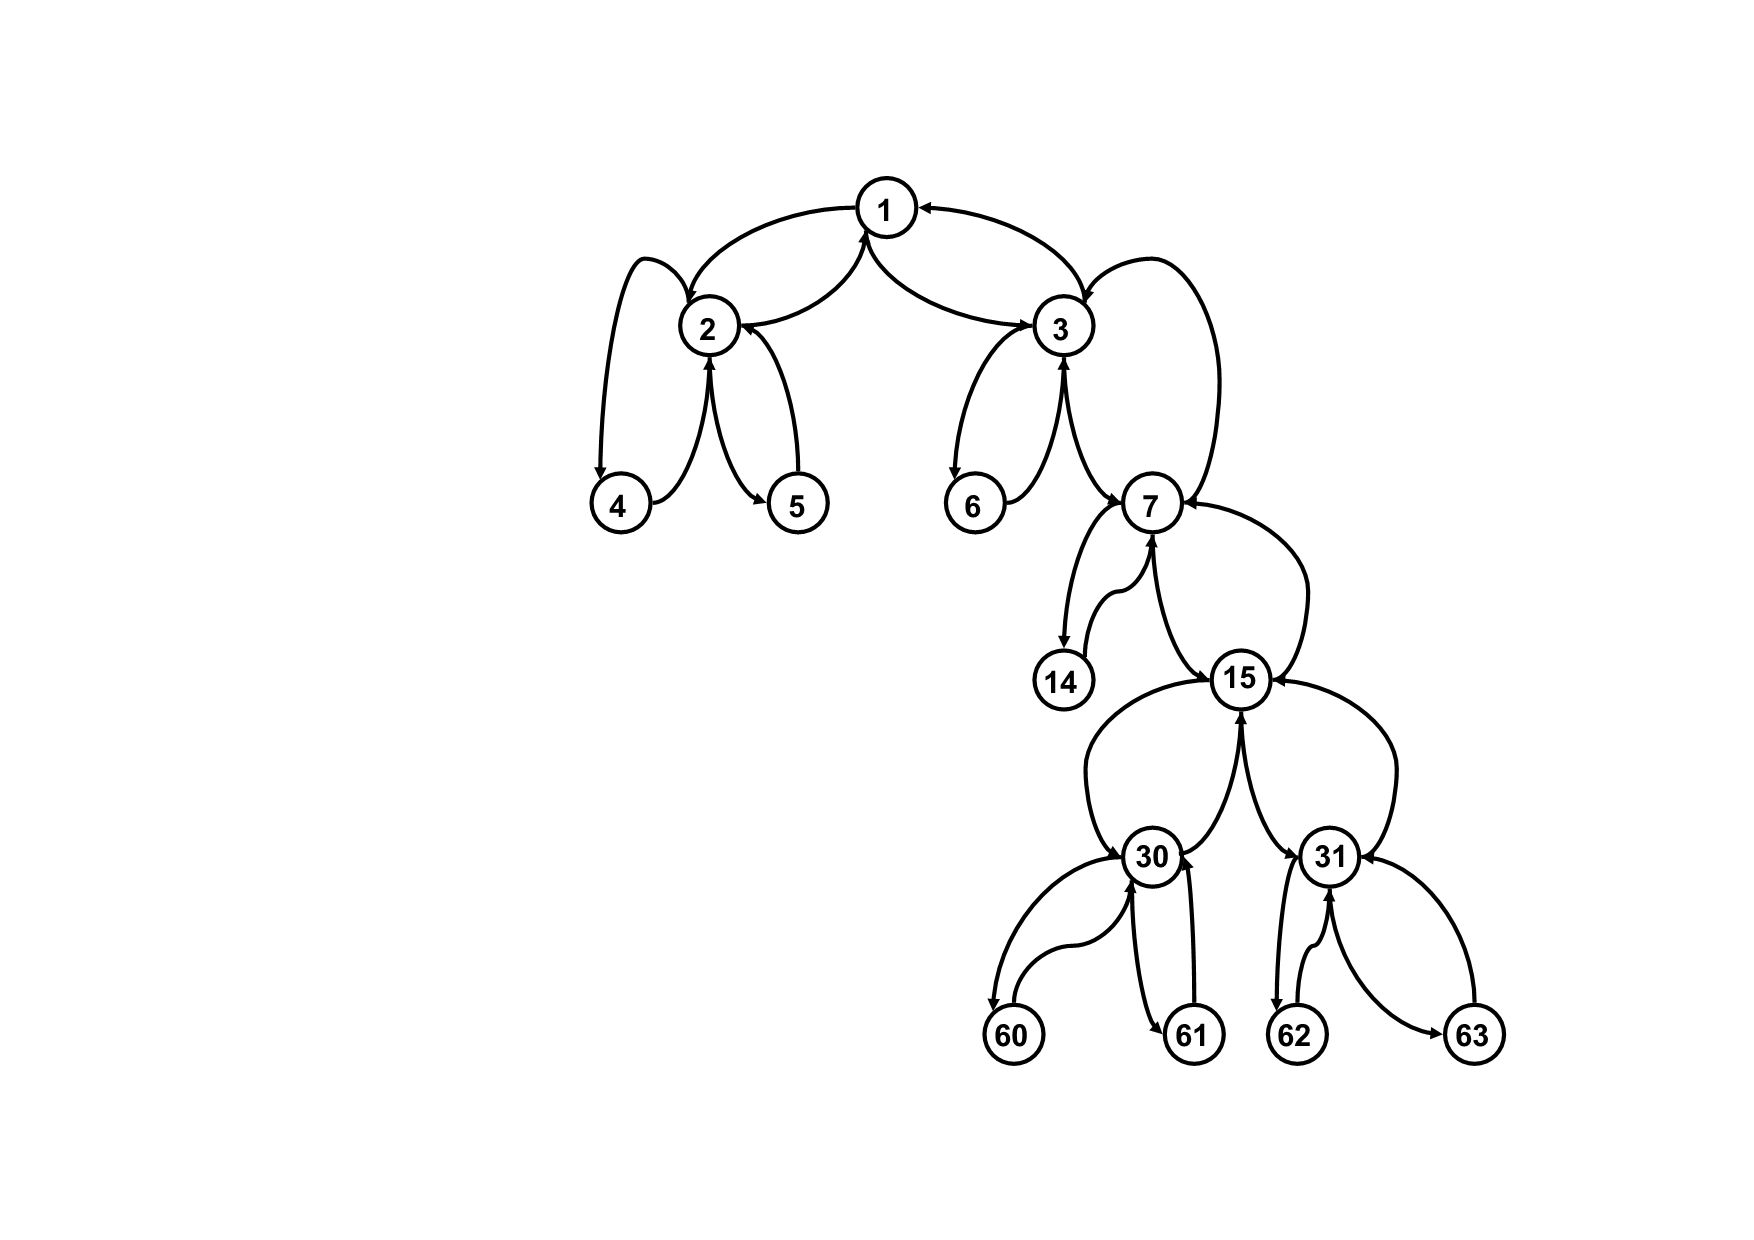
\includegraphics[width=\textwidth]{tree_graph}
	\caption{Illustration of how we go through the nodes for $tol=0.01$ to do Adaptive Simpson Integration without recursion.}
	\label{fig: tree}
\end{figure}

We ran the program with tolerance of $tol=10^{-2}, 10^{-3}, 10^{-4}$ and compared it to the value provided by Matlab. The outputs from the program is written below.
\newline

Output for a tolerance of $10^{-2}$
\begin{center}
\begin{lstlisting}
ASI: I = 2.505996157240214
Matlab: I = 2.500809110336167
Tol: 0.01000
\end{lstlisting}
\end{center}

Output for a tolerance of $10^{-3}$
\begin{center}
\begin{lstlisting}
ASI: I = 2.499856554302364
Matlab: I = 2.500809110336167
Tol: 0.00100
\end{lstlisting}
\end{center}

Output for a tolerance of $10^{-4}$
\begin{center}
\begin{lstlisting}
ASI: I = 2.500809666749028
Matlab: I = 2.500809110336167
Tol: 0.00010
\end{lstlisting}
\end{center}

\subsubsection*{Code for task 2}
\lstinputlisting[language=C++]{../pro1_t2.cpp}

\newpage
%test some code snippets
\begin{center}
\begin{minipage}[t]{85mm}
\begin{lstlisting}
for (int i=0; i<iterations;i++)
{
  do something
}
\end{lstlisting}
\end{minipage}
\end{center}

%\newpage
%\lstinputlisting[language=C++]{../pro1_t1.cpp}

\end{document}





